% ****** Start of file apssamp.tex ******
%
%   This file is part of the APS files in the REVTeX 4.1 distribution.
%   Version 4.1r of REVTeX, August 2010
%
%   Copyright (c) 2009, 2010 The American Physical Society.
%
%   See the REVTeX 4 README file for restrictions and more information.
%
% TeX'ing this file requires that you have AMS-LaTeX 2.0 installed
% as well as the rest of the prerequisites for REVTeX 4.1
%
% See the REVTeX 4 README file
% It also requires running BibTeX. The commands are as follows:
%
%  1)  latex apssamp.tex
%  2)  bibtex apssamp
%  3)  latex apssamp.tex
%  4)  latex apssamp.tex
%
\documentclass[%
 reprint,
nofootinbib,
%superscriptaddress,
%groupedaddress,
%unsortedaddress,
%runinaddress,
%frontmatterverbose,
%preprint,
%showpacs,preprintnumbers,
%nofootinbib,
%nobibnotes,
%bibnotes,
aps,
%pra,
%prb,
%rmp,
%prstab,
%prstper,
%floatfix,
]{revtex4-1}

\usepackage[utf8]{inputenc}
\usepackage[english]{babel}
\usepackage{dsfont}
\usepackage{amsmath}
\usepackage{amssymb}
\usepackage{graphicx}% Include figure files
\usepackage{dcolumn}% Align table columns on decimal point
\usepackage{bm}% bold math
\usepackage{amsmath}
\usepackage{varioref}
\usepackage{booktabs}
\usepackage[bottom]{footmisc}

\usepackage{algpseudocode}
\usepackage{listings}

\usepackage{tikz}

\newcommand{\RN}[1]{%
  \textup{\uppercase\expandafter{\romannumeral#1}}%
}


\newcolumntype{C}{>{$}c<{$}}
\AtBeginDocument{
\heavyrulewidth=.08em
\lightrulewidth=.05em
\cmidrulewidth=.03em
\belowrulesep=.65ex
\belowbottomsep=0pt
\aboverulesep=.4ex
\abovetopsep=0pt
\cmidrulesep=\doublerulesep
\cmidrulekern=.5em
\defaultaddspace=.5em
}

%\usepackage{hyperref}% add hypertext capabilities
%\usepackage[mathlines]{lineno}% Enable numbering of text and display math
%\linenumbers\relax % Commence numbering lines

%\usepackage[showframe,%Uncomment any one of the following lines to test
%%scale=0.7, marginratio={1:1, 2:3}, ignoreall,% default settings
%%text={7in,10in},centering,
%%margin=1.5in,
%%total={6.5in,8.75in}, top=1.2in, left=0.9in, includefoot,
%%height=10in,a5paper,hmargin={3cm,0.8in},
%]{geometry}

\begin{document}

%\preprint{APS/123-QED}

\title{Eigenvalue problems in pyhsics:\\
Solving the Schrödinger equation}% Force line breaks with \\

\author{Cecilie Glittum}\homepage{http://www.github.uio.no/cecilgl/FYS4150}
\author{Ivar Svalheim Haugerud}\homepage{http://www.github.uio.no/ivarsh/FYS4150}

\affiliation{%
 Department of Physics, University of Oslo\\
}%


\date{\today}% It is always \today, today,
             %  but any date may be explicitly specified

\begin{abstract}
In this article we study eigenvalue and eigenvector problems numerically using Jacobi's method. We study three different physical cases: The buckling beam and quantum dots with both one and two electrons. These physical systems are quite different, but the equations we need to solve are almost identical. We discretize the continuous equations, and use Jacobi's method to find the eigenvalues and eigenvectors of the systems. We find that Jacobi's method is not the best suited algorithm for tridiagonal matrices since the number of FLOPS goes as $n^4$. When studying quantum dots we compare our eigenvalues with analytical results to check if they are compatible. For the calculation we have to define an upper bound for our position vector to achieve correct eigenvalues. To find the ideal value of $\rho_{max}$ we use the analytical eigenvalues and run our simulation for different values of $\rho$ and $n$ and chose the best value. For the single electron case we find $\rho_{ideal}=4.65(5)$, and for two electrons the ideal value depends on the steepness of the potential. Studying the eigenvectors we extract important information of the interactions between two electrons in a quantum dot. Quantum dots are of wide interest, with many different applications, and to understand the energies and wavefunctions are important for many of the applications.
\end{abstract}


\maketitle


\section{Introduction}

Eigenvalue problems are often occurring in physics, in many different contexts. They are especially important in quantum mechanics, where the eigenfunctions and eigenvalues play a key role in the theory.\\
In this article we study first the eigenvalue problem of a buckling beam, before we look into quantum mechanics and quantum dots in three dimensions. We will study quantum dots for both one-electron and two-electron systems.\\
Even though the buckling beam and the single electron in a harmonic oscillator potential are drastically different physical objects, we will see that the equations which need to be solved are identical, except for some constant. For the two electron case we need to add some terms in the potential, but as we will see, the discretized equations has the same form. Because of this we can use Jacobi's method for all the systems we study.\par
The quantum dot (QD) is a hot topic of resarch. Because their highly tunable properties QDs are of wide interest. Potential applications include transistors, solar cells, LEDs, diode lasers, quantum computing, and medical imaging \cite{Q_DOTS}. To understand quantum dots is therefore important for many different applications. We will study the wave function and the energy eigenvalues of both one and two electrons in a three dimensional quantum dot.\par

Eigenvalue problems are solved numerically by discretizing the continuous functions, which makes the eigenvalue problem a linear algebra problem. Analytically, matrix eigenvalue problems are solved by calculating a determinant of same dimensions as the matrix, using Cramer's rule. Cramer's rule is computationally very expensive, e.g. the number of FLOPS needed for calculating a $6 \times 6$ determinant $\sim 2000$FLOPS, and it increases as $n!$. Therefore, we solve the eigenvalue problems diagonalizing the matrices with Jacobi's method, which is an iterative method. This means the algorithm will continue to run until a condition, specified by us, is satisfied. The algorithm will run until the matrix is almost diagonal, where every non diagonal element is effectively zero. We will discuss the usefulness of this algorithm for our problem. \\
All the physical systems we study have analytical solutions. This gives us the possibility to test our numerical results against the theoretical ones. This will prove to be especially important when deciding the maximum value of position for our algorithm, in the quantum mechanical case.\\
It is important to write clean code. We will therefore use unit-tests to control our programs, and make sure that changes in functions do not change the results. To do this we construct problems with known analytical solutions, which can be tested versus the numerical results produced by our algorithms.\par
\par
In this article we will go through the algorithms used, the results they produced, and discuss the results, before concluding on our work.


\section{Algorithms}

\subsection{Jacobi's method for solving eigenvalue problems}

To diagonalize matrices, we will use Jacobi's method. This method consists of a number of successive rotations in various hyperplanes, where in each rotation, we zero out two off-diagonal elements. We have specialized the algorithm to the case of symmetric matrices.

A rotation is a unitary transformation, and preserves the orthogonality of eigenvectors. If we rotate a coordinate system with the matrix $\hat{U}$, the vectors are rotated
\begin{equation}
\vec{x}_i \rightarrow \vec{x}_i^\prime = \hat{U}^T\vec{x}_i.
\end{equation}
The corresponding transformation of operators/matrices is then
\begin{equation}
\hat{A} \rightarrow \hat{A}^\prime = \hat{U}^T\hat{A}\hat{U}.
\end{equation}
We can show that this transformation of $\vec{x}_i$ preserves the orthogonality:
\begin{align}
\vec{x}_i^\prime\cdot\vec{x}_j^\prime &= \vec{x}_i^{\prime T}\vec{x}_j^\prime\\
&= (\hat{U}^T\vec{x}_i)^T\hat{U}^T\vec{x}_j\\
&= \vec{x}_i^T\hat{U}\hat{U}^T\vec{x}_j\\
&= \vec{x}_i^T\vec{x}_j\\
&= \vec{x}_i\cdot \vec{x}_j,
\end{align}
such that the dot product and orthogonality (if $\vec{x}_i\cdot \vec{x}_j = \delta_{ij}$) is preserved.

Jacobi's method is built upon the fact that the Fröbenius norm of a matrix is conserved under orthogonal transformations\cite{hjorten}. The Fröbenius norm of a matrix $\hat{A}$ is defined as
\begin{equation}
\lvert\lvert\hat{A}\rvert\rvert_F^2 = \sum_{ij} \lvert a_{ij}\rvert ^2,
\end{equation}
where $a_{ij}$ are the elements of the matrix.

Let $\hat{B}$ be the result when $\hat{A}$ is transformed under an orthogonal transformation $\hat{S}$, i.e.
\begin{equation}
\hat{B} = \hat{S}^T\hat{A}\hat{S}.
\end{equation}
Then $\lvert\lvert\hat{B}\rvert\rvert_F^2 = \lvert\lvert\hat{A}\rvert\rvert_F^2$. The sums of the off-diagonal elements are
\begin{align}
\mathrm{off}(\hat{A}^2) &= \lvert\lvert\hat{A}\rvert\rvert_F^2 - \sum_i a_{ii}^2\\
\mathrm{off}(\hat{B}^2) &= \lvert\lvert\hat{A}\rvert\rvert_F^2 - \sum_i b_{ii}^2
\end{align}
Since we zero out two elements on the off-diagonal by doing the transformation, it can be shown in the $2\times 2$ case that
\begin{equation}
\mathrm{off(\hat{B}^2)} = \mathrm{off(\hat{A}^2)} -2a_{kl},
\end{equation}
where $b_{kl}$ is the element that is zeroed out. Generalizing this, we see that by picking the largest $a_{kl}$, we get the smallest value for $\mathrm{off}(\hat{B}^2)$. When the matrix is diagonalized, the sum of the off-diagonal elements is obviously zero.

To choose the axis to rotate about, we therefore need to find the indices of the biggest off-diagonal element of the matrix. Since our matrix is symmetric, we only search through the upper off-diagonal of the matrix. When we have found the indices $k$ and $l$ of the biggest off-diagonal element, we can define the orthogonal transformation as
\begin{equation}
\hat{S} =
\begin{bmatrix}
1 & 0 & \dots & 0 & 0 & \dots & 0 & 0\\
0 & 1 & \dots & 0 & 0 & \dots & 0 & 0\\
\vdots & \vdots & \vdots & \vdots & \vdots & \vdots & \vdots & \vdots\\
0 & 0 & \dots & \cos\theta & 0 & \dots & 0 & \sin\theta\\
0 & 0 & \dots & 0 & 1 & \dots & 0 & 0\\
\vdots & \vdots & \vdots & \vdots & \vdots & \ddots & \vdots & \vdots\\
0 & 0 & \dots & 0 & 0 & \dots & 1 & 0\\
0 & 0 & \dots & -\sin\theta & 0 & \dots & 0 & \cos\theta
\end{bmatrix}
\end{equation}
with $s_{kk} = s_{ll} = \cos\theta, s_{kl} = -s_{lk} = \sin\theta, s_{ii} = 1 \quad i \neq l, k$.

We have to decide the value of $\theta$ so that
\begin{equation}
b_{kl} = (a_{kk} -a_{ll})\cos\theta\sin\theta + a_{kl}(\cos^2\theta - \sin^2\theta) = 0.
\end{equation}
This equation can be rewritten by dividing all terms by $a_{kl}\cos^2\theta$, which gives
\begin{equation}\label{eq: t-equation}
t^2 + 2\tau t - 1 = 0,
\end{equation}
where $t = \tan\theta$ and
\begin{equation}
\tau = \frac{a_{ll}-a_{kk}}{2a_{kl}}.
\end{equation}
Solving Eq. \eqref{eq: t-equation} for $t$ gives
\begin{equation}
t = -\tau \pm \sqrt{1 + \tau^2},
\end{equation}
which can be rewritten as
\begin{equation}
t = \frac{1}{\tau \pm \sqrt{1 + \tau^2}},
\end{equation}
where we choose $+(-)$ for $\tau$ positive(negative). In this way, we both ensure that we don't subtract two almost equal numbers, as well as we choose the smallest value for $t$ to ensure that none of the other matrix elements blow up during the rotations\cite{hjorten}.

We can now get $c = \cos\theta$ and $s = \sin\theta$ by
\begin{align}
c &= \frac{1}{\sqrt{1 + t^2}}\\
s &= ct.
\end{align}

Only a few matrix elements change by the transformation $\hat{A} \rightarrow \hat{S}^T\hat{A}\hat{S}$. When multiplying $\hat{A}$ with $\hat{S}^T$ from the left, only the rows $k$ and $l$ are affected and change to
\begin{align}
\hat{A}_{ki} &= c\hat{A}_{ki} - s\hat{A}_{li},\\
\hat{A}_{li} &= s\hat{A}_{ki} + c\hat{A}_{li}.
\end{align}
When we then multiply the resulting matrix $(\hat{S}^T\hat{A})$ with $\hat{S}$ from the right, only the columns $k$ and $l$ are affected and change to
\begin{align}
\hat{A}_{ik} &= c\hat{A}_{ik} - s\hat{A}_{il},\\
\hat{A}_{il} &= s\hat{A}_{ik} + c\hat{A}_{il}.
\end{align}

Now, we have everything we need to do the transformations. We continue doing transformations until
\begin{equation}
  \text{max}(a_{ij}^2) \leq \epsilon \label{off_A}, \qquad j<i
\end{equation}
then we say that our matrix is diagonalized. The eigenvalues of the matrix $\hat{A}$ is then the diagonal elements of the diagonal matrix $\hat{D}$. If we must do $N$ transformations to diagonalize the matrix, we have
\begin{equation}
\hat{D} = \hat{S}^T_N ... \hat{S}^T_2 \hat{S}^T_1\hat{A} \hat{S}_1\hat{S}_2...\hat{S}_N
\end{equation}
On the eigenvectors $\hat{x}$ (where $\hat{x}$ is the matrix containing the eigenvectors of $\hat{A}$ as its columns), we have then
\begin{equation}
\mathds{1} = \hat{S}^T_N...\hat{S}^T_2\hat{S}^T_1\hat{x},
\end{equation}
since the eigenvectors for $\hat{D}$ are the vectors $\vec{e_i}$, thus we can find the eigenvectors by
\begin{equation}
\hat{x} = \hat{S}_1\hat{S}_2...\hat{S}_N.
\end{equation}
The column $i$ of $\hat{x}$ is the eigenvector of $\hat{A}$ with eigenvalue $d_{ii}$.

The complete algorithm for computing the eigenvalues and eigenvectors are then for $\hat{A} \in \mathds{R}^{n\times n}$
\begin{algorithmic}[H]
\State
\State Initialize matrix $\hat{R}$ as identity matrix;
\State choose tolerance $\epsilon$
\While {max$(a_{ij}^2) > \epsilon$}
	\State find $k,l$, where $\lvert a_{kl}\rvert = $max$_{i\neq j}\lvert a_{ij}\rvert$;
	\State compute $\tau$;
	\If {$\tau > 0$}
		\State $t = 1/(\tau + \sqrt{1 + \tau^2})$;
	\EndIf
	\If {$\tau < 0$}
		\State $t = 1/(\tau - \sqrt{1 + \tau^2})$;
	\EndIf
	\State compute c, s;
	\For {i = 0, 1, ..., n-1} \Comment Compute $\hat{S}^T\hat{A}$
		\State Aki = $A_{ki}$;
   		\State  Ali = $A_{li}$;
   		\State $A_{ki}$ = Aki*c - Ali*s;
   		\State $A_{li}$ = Aki*s + Ali*c;
	\EndFor
	\For {i = 0, 1, ..., n-1} \Comment Compute $(\hat{S}^T\hat{A})\hat{S}$
		\State Aik = $A_{ik}$;
   		\State Ail = $A_{il}$;
   		\State $A_{ik}$ = Aik*c - Ail*s;
   		\State $A_{il}$ = Aik*s + Ail*c;
	\EndFor
	\For {i = 0,1, ..., n-1} \Comment Compute eigenvectors
		\State Rik = $R_{ik}$;
    		\State Ril = $R_{il}$;
     	\State $R_{ik}$ = Rik*c - Ril*s;
    		\State $R_{il}$ = Rik*s + Ril*c;
	\EndFor
\EndWhile
\State
\end{algorithmic}

We will implement the part computing the eigenvalues and eigenvectors in two separate functions, which is inefficient if we want both, but is faster if we only want the eigenvalues.


\subsection{Classical mechanics: Buckling beam}

The first eigenvalue problem we look at is a classical mechanics problem; a buckling beam. The vertical displacement of the beam in the $y$-direction (see Fig. \ref{fig: buckling beam}), $u(x)$ is given by the following differential equation
\begin{equation}\label{eq: buckeling beam unscaled}
\gamma \frac{d^2 u(x)}{dx^2} = -Fu(x),
\end{equation}
where $\gamma$ is a constant defined by properties like the rigidity of the beam and $F$ is a force applied at $(L,0)$ towards the origin. We solve this equation with Dirichlet boundary conditions: $u(0) = u(L) = 0$.

\begin{figure}
\centering
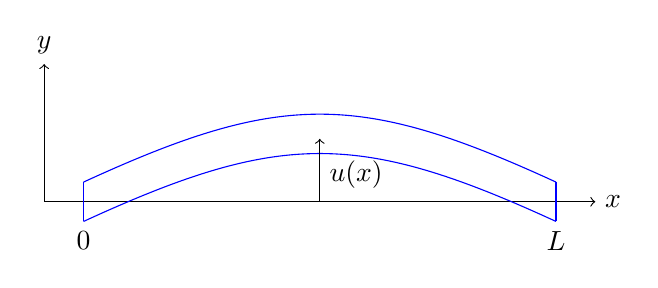
\begin{tikzpicture}
\draw [->] (0,0) -- (7,0);
\node at (7,0) [right] {$x$};

\draw [->] (0,0) -- (0,1.75);
\node at (0,1.75) [above] {$y$};

\draw [blue] (0.5,-0.25) -- (0.5,0.25);
\draw [blue] (6.5,-0.25) -- (6.5,0.25);

\draw [blue] (0.5,0.25) .. controls (3,1.4) and (4, 1.4) .. (6.5,0.25);
\draw [blue] (0.5,-0.25) .. controls (3,0.9) and (4, 0.9) .. (6.5,-0.25);

\draw [->] (3.5, 0) -- (3.5, 0.8);
\node at (3.5, 0.35) [right] {$u(x)$};

\node at (0.5, -0.25) [below] {$0$};
\node at (6.5, -0.25) [below] {$L$};

\end{tikzpicture}

\caption{A buckling beam fastened at both ends. The vertical displacement of the beam in the $y$-direction is given by $u(x)$. The boundary conditions are $u(0) = u(L) = 0$.}
\label{fig: buckling beam}
\end{figure}

We want to scale the equation to be able to work with reasonable numbers. We assume the values for $\gamma$, $F$ and $L$ to be known, and define the dimensionless variable
\begin{equation}
\rho = \frac{x}{L},
\end{equation}
where $\rho \in [0,1]$. This gives $dx \rightarrow Ld\rho$, which means that Eq. \eqref{eq: buckeling beam unscaled} can be rewritten as the dimensionless equation

\begin{equation}
\frac{d^2 u(\rho)}{d\rho^2} = -\frac{FL^2}{\gamma} u(\rho) = -\lambda u(\rho),
\end{equation}
where $\lambda = FL^2/\gamma$. This dimensionless eigenvalue problem can be solved numerically by discretizing. We discretize in the same way as C. Glittum and I. Haugerud\cite{project1}. This leaves us with
\begin{equation}
-\frac{u_{i+1} + u_{i-1} -2u_i}{h^2} = \lambda u_i,
\end{equation}
where $h$ is the step length, in this case $h = \frac{1-0}{n+1} = \frac{1}{n+1}$ because $i \in \{0,1,2, ..., n, n+1\}$.  We can rewrite this as a set of linear equations, which again can be written as a matrix eigenvalue problem of a tridiagonal Toeplitz matrix.
\begin{equation}\label{eq: matrix}
\begin{bmatrix}
d & e & 0 & 0 & 0 & \dots & 0\\
e & d & e & 0 & 0 & \dots & 0\\
0 & e & d & e & 0 & \dots & 0\\
\dots & \dots & \dots & \dots & \dots & \dots & \dots &\\
0 & \dots & \dots & \dots & e & d & e\\
0 & \dots & \dots & \dots & \dots & e & d
\end{bmatrix}
\begin{bmatrix}
u_1\\
u_2\\
u_3\\
\vdots\\
u_{n-1}\\
u_{n}
\end{bmatrix}
 =
 \lambda
 \begin{bmatrix}
u_1\\
u_2\\
u_3\\
\vdots\\
u_{n-1}\\
u_{n}
\end{bmatrix}
\end{equation}

The endpoints ($u_0$ and $u_{n+1}$) are left out as they are set to zero by the boundary conditions. In our case $d = 2/h^2$ and $e = -1/h^2$, but in general this tridiagonal Toeplitz matrix has analytical eigenpairs, with eigenvalues
\begin{equation}\label{eq: anal eigenvals}
\lambda_j = d + 2e\cos\left(\frac{j\pi}{n+1}\right), \quad j = 1, 2, ..., n.
\end{equation}
Thus, we implement Jacobi's method and test our results against the analytical eigenvalues given by Eq. \eqref{eq: anal eigenvals} by writing a unit-test. We also study the number of iterations needed to diagonalize the matrix as a function of the matrix size $n$ by implementing an iteration-counter in our Jacobi's method.


\subsection{Quantum mechanics: Quantum dots in three dimensions}

\subsubsection{One electron}

We look at electrons in a harmonic oscillator potential: $V(r) = \frac{1}{2}kx^2 = \frac{1}{2}m\omega^2x^2$. This potential is spherical symmetric, and thus the Schrödinger equation is separable into $\psi(r, \theta, \phi) = R(r)Y^m_l(\theta, \phi)$. After separation of variables, the radial part of the Schrödinger equation reads
\begin{equation}
  -\frac{\hbar^2}{2 m} \left ( \frac{1}{r^2} \frac{d}{dr} r^2
  \frac{d}{dr} - \frac{l (l + 1)}{r^2} \right )R(r)
     + V(r) R(r) = E R(r),
\end{equation}
where $r \in [0, \infty]$. The energies of the three dimensional harmonic oscillator are
\begin{equation}\label{eq: HO energy}
E_{nl}=  \hbar \omega \left(2n+l+\frac{3}{2}\right),
\end{equation}
with $n=0,1,2,\dots$ and $l=0,1,2,\dots$.

We want the radial Schrödinger equation to be rewritten as an eigenvalue equation including the double derivative. We therefore define $u(r) = rR(r)$, which gives
\begin{equation}
  -\frac{\hbar^2}{2 m} \frac{d^2}{dr^2} u(r)
       + \left ( V(r) + \frac{l (l + 1)}{r^2}\frac{\hbar^2}{2 m}
                                    \right ) u(r)  = E u(r) .
\end{equation}
We need the wave function to be finite at $r = 0$ and go to zero as $r$ approaches infinity. This implies that $u(0) = u(\infty) = 0$.

Now, we  only need to scale the equation:
As in the case of the buckling beam, we introduce a dimensionless variable $\rho = r/\alpha$, where $\alpha$ has unit length. Our equation is then
\begin{equation}
  -\frac{\hbar^2}{2 m \alpha^2} \frac{d^2}{d\rho^2} u(\rho)
       + \left ( V(\rho) + \frac{l (l + 1)}{\rho^2}
         \frac{\hbar^2}{2 m\alpha^2} \right ) u(\rho)  = E u(\rho) .
\end{equation}
We will in this article set $l=0$.  In terms of $\rho$ our harmonic oscillator potential is $V(\rho) = \frac{1}{2}k\alpha^2\rho^2$. Inserting this, we get
\begin{equation}
  -\frac{\hbar^2}{2 m \alpha^2} \frac{d^2}{d\rho^2} u(\rho)
       + \frac{k}{2} \alpha^2\rho^2u(\rho)  = E u(\rho) .
\end{equation}
We still have a unit $\mathrm{energy}/\mathrm{length}^2$ in the coefficients of the equation. To scale the equation, we divide it by $\hbar^2/(2 m \alpha^2)$, which gives
\begin{equation}
  -\frac{d^2}{d\rho^2} u(\rho)
       + \frac{mk}{\hbar^2} \alpha^4\rho^2u(\rho)  = \frac{2m\alpha^2}{\hbar^2}E u(\rho) .
\end{equation}
The constant $\alpha$ can now be fixed so that
\begin{equation}
\frac{mk}{\hbar^2} \alpha^4 = 1 \Rightarrow
\alpha = \left(\frac{\hbar^2}{mk}\right)^{1/4}.
\end{equation}
Defining
\begin{equation}\label{eq: lambda}
\lambda = \frac{2m\alpha^2}{\hbar^2}E,
\end{equation}
we can rewrite Schrödinger's equation as
\begin{equation}\label{eq: scaled one electron schro}
  -\frac{d^2}{d\rho^2} u(\rho) + \rho^2u(\rho)  = \lambda u(\rho).
\end{equation}

Thus the Schrödinger equation for one electron in a 3D harmonic oscillator potential is reduced to an eigenvalue problem which we can solve by disretizing Eq. \eqref{eq: scaled one electron schro}. The discretized equation is
\begin{equation}
-\frac{u_{i+1} -2u_i +u_{i-1}}{h^2}+\rho_i^2u_i = \lambda u_i.
\end{equation}
By defining
\begin{align}
d_i &= \frac{2}{h^2} + \rho_i^2\\
e_i &= -\frac{1}{h^2},
\end{align}
we get
\begin{equation}
e_i u_{i-1} + d_i u_i + e_iu_{i+1} =  \lambda u_i.
\end{equation}
This corresponds to the same matrix eigenvalue problem as in Eq. \eqref{eq: matrix}, and we will solve it by Jacobi's method to obtain both the eigenvalues and eigenstates of one electron in a harmonic oscillator potential.

The analytical eigenvalues are in this case given by Eqs. \eqref{eq: HO energy} and \eqref{eq: lambda}, which together give $\lambda = 3, 7, 11, 15, \dots$.

When working with the harmonic oscillator potential we need to define a maximum value of $\rho$, as $\rho = \infty$ is not applicable numerically.\\To find the ideal value of $\rho$ we calculate the first three eigenvalues, and compute their difference with the analytical ones. We do this for different values of both $n$ and $\rho_{max}$ and compute the average deviation for each $\rho_{max}$ and $n$. In this way, we can find the optimal combination of $n$ and $\rho_{max}$.


\subsubsection{Two electrons}

Lastly, we look at two electrons in a three dimensional harmonic oscillator potential, and include  interactions between the electrons in the form of repulsive Coulomb interactions. The Schrödinger equation for two electrons in a harmonic oscillator potential with no interactions is
\begin{equation}
\left(  -\frac{\hbar^2}{2 m} \frac{d^2}{dr_1^2} -\frac{\hbar^2}{2 m} \frac{d^2}{dr_2^2}+ \frac{1}{2}k r_1^2+ \frac{1}{2}k r_2^2\right)u(r_1,r_2)  = E^{(2)} u(r_1,r_2),
\end{equation}
where $E^{(2)}$ is the two-electron energy. When the electrons are not interacting, we can write $u(r_1, r_2) = u(r_1)u(r_2)$. We can rewrite the Schrödinger equation in terms of the center-of-mass coordinate $\vec{R} = (\vec{r}_1 + \vec{r}_2)/2$ and the relative coordinate $\vec{r} = \vec{r}_1 - \vec{r}_2$:
\begin{equation}
\left(  -\frac{\hbar^2}{m} \frac{d^2}{dr^2} -\frac{\hbar^2}{4 m} \frac{d^2}{dR^2}+ \frac{1}{4} k r^2+  kR^2\right)u(r,R)  = E^{(2)} u(r,R).
\end{equation}
This equation can be separated into one R-dependent equation and one r-dependent equation.

When including the repulsive Coulomb interaction between the two electrons, we must add a term to the potential energy
\begin{equation}
V(r_1,r_2) = \frac{\beta e^2}{|\mathbf{r}_1-\mathbf{r}_2|}=\frac{\beta e^2}{r},
\end{equation}
where $\beta e^2=1.44\mathrm{nmeV}$.

After separation of variables, the r-dependent Schrödinger equation with Coulomb interaction reads
\begin{equation}\label{eq: r-dependent Schrodinger}
\left(  -\frac{\hbar^2}{m} \frac{d^2}{dr^2}+ \frac{1}{4}k r^2+\frac{\beta e^2}{r}\right)\psi(r)  = E_r \psi(r).
\end{equation}
The full energy of the system is given by $E^{(2)} = E_r + E_R$. Eq. \eqref{eq: r-dependent Schrodinger} is a one-dimensional Schrödinger equation which we can scale and discretize to solve numerically.

We begin with scaling the equation. Like in the case for one electron, we define $\rho = r/\alpha$ and divide by $\hbar^2/m$. This turns Eq. \eqref{eq: r-dependent Schrodinger} into
\begin{equation}
  -\frac{d^2}{d\rho^2} \psi(\rho)
       + \frac{1}{4}\frac{mk}{\hbar^2} \alpha^4\rho^2\psi(\rho)+\frac{m\alpha \beta e^2}{\rho\hbar^2}\psi(\rho)  =
\frac{m\alpha^2}{\hbar^2}E_r \psi(\rho) .
\end{equation}
To simplify the equation further, we can define
\begin{equation}
\omega_r^2=\frac{1}{4}\frac{mk}{\hbar^2} \alpha^4,
\end{equation}
and fix $\alpha$ by requiring
\begin{equation}
\frac{m\alpha \beta e^2}{\hbar^2}=1.
\end{equation}
By doing so, our equation reads
\begin{equation}
  -\frac{d^2}{d\rho^2} \psi(\rho) + \omega_r^2\rho^2\psi(\rho) +\frac{1}{\rho}\psi(\rho) = \lambda \psi(\rho),
\end{equation}
where
\begin{equation}
\lambda = \frac{m\alpha^2}{\hbar^2}E_r.
\end{equation}

Now we have an equation which we can discretize. By doing so, we get
\begin{equation}\label{eq: two electrons discretized}
 -\frac{\psi_{i+1} -2\psi_i +\psi_{i-1}}{h^2} + \omega_r^2\rho_i^2\psi_i +\frac{1}{\rho_i}\psi_i = \lambda \psi_i.
\end{equation}
By defining
\begin{align}
d_i &= \frac{2}{h^2} + \omega_r^2\rho_i^2 + \frac{1}{\rho_i},\\
e_i &= -\frac{1}{h^2},
\end{align}
we get a set of linear equations described by the eigenvalue problem in Eq. \eqref{eq: matrix}, which we solve by Jacobi's method. We then find both the eigenvalues and eigenstates of the r-dependent Schrödinger equation for two interacting electrons in a harmonic oscillator potential.



\section{Results}

For the buckling beam, the unit-test ran sucessfully, meaning that our implemented Jacobi's method returned the correct eigenvalues in Eq. \eqref{eq: anal eigenvals} (up to a tolerance).

In Fig. \vref{fig:iterations_needed} we see how the number of iterations needed to satisfy \eqref{off_A} depends on the size $n$ of the matrix we're diagonalizing. The log-log plot shown in the figure has a slope of $2.02(1)$, which means that the number of iterations needed goes as $n^2$. This figure was generated with a tolerance of $\epsilon=10^{-7}$.\\
The number of FLOPS for each iteration is $n^2/2 + 11n + 13$ (where we have counted the if-test for finding $max(a_{kl}^2)$ as one flop, because it uses CPU-time). This results in the total number of FLOPS being approximately proportional to the size of the matrix to the power of four.

\begin{figure}
\centering
\includegraphics[scale=0.5]{../figures/iterations_needed.pdf}
\caption{Iterations needed to diagonalize a matrix using Jacobi's method, here plotted as a function of matrix size $n$, with a tolerance of $\epsilon=10^{-7}$ to reach the condition requirement of the the largest non-diagonal element being smaller than $\epsilon$.}
\label{fig:iterations_needed}
\end{figure}

The results we found when studying the optimal value of $\rho_{max}$ is shown in Fig. \vref{fig:deviation_n_rho}. We find that the optimal value of $\rho_{max}$ is $4.65(5)$.
\par

\begin{figure}
\centering
\includegraphics[scale=0.5]{../figures/rho_vs_n.pdf}
\caption{The logarithm of the average deviation between the analytical and numerical results for the first three eigenvalues of one electron in a harmonic oscillator potential.}
\label{fig:deviation_n_rho}
\end{figure}

\begin{table}[]
\caption{Energy eigenvalues for one electron in a harmonic oscillator potential. The numerically found values using Jacobi's method are compared to the analytical ones. All examples were run with $\rho_{max}=4.65$ for a $200\times 200$ matrix.}
\begin{tabular}{@{}llll@{}}
\toprule
Eigenvalue \# & Analytical & Numerical & Relative deviation\\ \midrule
0     & $3$       & 2.99983  &  $5.6\times10^{-5}$    \\
1     & $7$       & 6.99921  &  $1.3\times10^{-4}$   \\
2     & $11$      & 11.0006  &  $5.4\times10^{-5}$ \\
3     & $15$      & 15.0439  &  $2.9\times10^{-3}$   \\
4     & $19$      & 19.3448  &  $1.8\times10^{-2}$   \\
\botrule
\end{tabular}
\label{table:one_ele}
\end{table}

The energies found for the single electron in a harmonic oscillator potential are given in table \ref{table:one_ele}. The normalized probability densities for the three lowest energy states are shown in Fig. \vref{fig:one_e_prob_density}.
The precision when calculating the energy eigenvalues depend on the size of the matrix. The size needed for a specific precision depends on the eigenvalue number. To reach an accuracy of four leading digits, it requierd too large computational time for energy eigenvalues outside the ground state. For the ground state it requierd a matrix size of $270$ to reach a precision of four leading digits. For the larger eigenvalues we calculated the size needed, in increments of $10$, to reach an accuracy of $10^{-3}$, the results are shown in table \ref{table:accuracy}.

\begin{table}[]
\caption{The size of the matrix needed to reach a deviation of $10^{-3}$ for different eigenvalues. This was calculated with a size increment of $10$.}
\begin{tabular}{@{}lllll@{}}
\toprule
Eigenvalue \# &  $\rho_{max}$ & Analytical & Numerical & Matrix size\\ \midrule
0     & $4.65$ & $3$       &  2.9992   &  $90$     \\
1     & $4.65$ & $7$       &  6.9991   &  $190$    \\
2     & $4.65$ & $11$      & 10.9990   &  $200$    \\
3     & $5.5$  & $15$      & 14.9993   &  $430$    \\
\botrule
\end{tabular}
\label{table:accuracy}
\end{table}


\begin{figure}
  \centering
  \includegraphics[scale=0.5]{../figures/wavefunc_one_e.pdf}
  \caption{Solution of the radial equation of the three lowest energy eigenstates for one electron in a harmonic oscillator potential as function of the scaled position $\rho$. Here, we have used $\rho_{max} = 4.65$.}
  \label{fig:one_e_prob_density}
\end{figure}


When we introduce a second electron in our system and study the ground state, with the azimuthal quantum number $l$ set to zero, we get the results shown in table \vref{table:eigenvalues}. Due to the theoretical work of M. Taut\cite{PhysRevA.48.3561} we can compare the numerically found eigenvalues with the analytical ones.
\\For the two electrons we calculated the probability density for the ground state as a function of  relative distance between the electrons, for the specific values of the oscillator-parameter $\omega_r$, this is shown in Fig. \vref{fig:many_omega}. \\
The effect of the Coloumb interaction is shown in Fig. \vref{fig:compare} where the ground state is shown for the single and two electron case, with $\omega_r=1.0$.

\begin{table}[]
\caption{Eigenvalues for different values of $\omega_r$. The analytical eigenvalues by M. Taut\cite{PhysRevA.48.3561} are compared to the numerical found by Jacobi's method with the given $\rho_{max}$.}
\begin{tabular}{@{}lllll@{}}
\toprule
$\omega$ & $\rho_{max}$ & Analytical & Numerical & Relative deviation \\ \midrule
0.25     & 10   \qquad \quad       & 1.25      & 1.24997 &  $2.4\times 10^{-5}$  \\
0.05     & 20           & 0.35       & 0.349997 &  $8.4\times 10^{-6}$ \\
0.01827\qquad  \,  & 30           & 0.1644  \qquad \quad   & 0.164441 & $2.5\times 10^{-4}$  \\ \botrule
\end{tabular}
\label{table:eigenvalues}
\end{table}


\begin{figure}
\centering
\includegraphics[scale=0.5]{../figures/wavefunc_many_omega.pdf}
\caption{Solution of the radial equation of the ground state of the two interacting electrons in a harmonic oscillator potential for different values of $\omega_r$. These  probability densities are found numerically using Jacobi's algorithm. The position coordinate is the scaled relative distance between the two electrons. Note that we have a logarithmic axis for $\rho$.}
\label{fig:many_omega}
\end{figure}



\begin{figure}
\centering
\includegraphics[scale=0.5]{../figures/difference_interaction.pdf}
\caption{Solution of the radial equation of the ground state of the two interacting electrons in a harmonic oscillator potential for $\omega_r=1$ with the single electron case in a harmonic oscillator potential. These  probability densities are found numerically using Jacobi's algorithm. The position coordinate is the scaled relative distance between the two electrons. }
\label{fig:compare}
\end{figure}

\section{Discussion}

Jacobi's method is an iterative method. Thus it will continue to run until a condition set by to program is satisfied. For our case the statement which has to be satisfied is equation \eqref{off_A}. For each iteration we multiply our $n\times n$ matrix by two other $n\times n$ matrices. Therefore the number of iterations should depend on the size of the matrix used.%, and we see that the number of iterations goes as $n^2$ in Fig. \ref{fig:iterations_needed}.

 As we see in Fig. \vref{fig:iterations_needed} the number of iterations for  Jacobi's method goes as $n^2$. Since the number of FLOPS per iteration goes as $n^2$, the total number of FLOPS goes as $n^4$. Because of this, Jacobi's method makes the upper bound for the matrix size quite small compared to other methods. Therefore we can not use large matrices. This is a problem. For finding the energy eigenvalue of the ground state, with four leading digits, we needed $270\times 270$ matrix, which since the number of FLOPS goes as $n^4$, takes a long time to calculate. And even worse for the energy eigenvalue of the second lowest energy eigenstate. Jacobi's method limits the precision of our eigenpairs, due to the required computational time.\par
%Since we will never actually reach exactly zero when using Jacobi's method, we need to define a tolerance for when we are satisfied with our iterative method. The eigenvalues we find will therefore not be exactly equal to the analytical eigenvalues. It is therefore important to test the numerical eigenvalues against the analytical eigenvalues within a tolerance.

For the one-electron case in an harmonic oscillator, we used the analytical eigenvalues to find an ideal value of $\rho_{max}$, the result is shown in Fig. \vref{fig:deviation_n_rho}. In theory $\rho_{max}$ should be infinite, but this is not possible for a computer, so we have to make a compromise. If we make $\rho$ too small the real wavefunction will get \textit{cut off} before it is practically zero. If we make $\rho$ too large, the precision of $\rho$ decreases, since $\Delta \rho$ increases if $n$ stays the same.
From Fig. \vref{fig:deviation_n_rho} we see that the deviation decreases as $n$ increases, as we would assume. But we also find a minima in the value for $\rho_{max}$ at $4.65(5)$. This is the ideal value of $\rho_{max}$ for the three lowest energy eigenstates. This would no longer be the case if we studied the higher energy eigenstates, since it more probable that the higher energy eigenstates are observed further from the origin, and therefore requiers a larger $\rho_{max}$.

As we can see from Fig. \vref{fig:one_e_prob_density} we are more likely to measure the position of the electron further from the origin for higher energy eigenstates. This is due to the energy of the state increasing, which gives the electron the possibility to climb further up the potential. Since the potential goes as $\omega^2r^2$, the increase of the potential is quite rapid. From the figure we can also see that the number of nodes increases linearly with the eigenstate number.

Much of the same apply in the two-electron case. The two electrons have the same charge, and want to distance them self from each other. This will force the probability densities further away from the origin, as we see in Fig. \ref{fig:compare}. Since the electrons live in a harmonic oscillator potential they will not be able to move infinitly far from each other, they are restricted by the potential. How far they are able to move away from each other is dependent on the steepness of the harmonic oscillator potential. The steepness of the potential increases with $\omega_r$ increases. When $\omega_r$ is small the potential is increasing slowly with $\rho$. This results in their wavefunction being able to get pushed further away from the origin, and their radial position will be more uncertain. When $\omega_r$ is large the potential increasis rapidly with $\rho$, and the electrons are not able to seperate from eachother as much. We can see that this clearly by comparing Fig. \ref{fig:one_e_prob_density} and Fig. \ref{fig:many_omega}, as well as in the comparison shown in Fig. \ref{fig:compare}. \par

From table \vref{table:one_ele} we see that the relative deviation between the analytical and numerical eigenvalues increase for the heigher energy eigenvalues. There are a couple of reasons for this. For the heigher energy eigenvalues the calculation should be done with larger $\rho_{max}$, and the results shown in this table was calculated with the same value of $\rho_{max}$ for all eigenvalues. The value of $\rho_{max}$ used was the ideal value for the three lowest energy eigenstates, which is not the ideal value for larger energy eigenstates. Another reason can be seen in table \ref{table:accuracy} where the needed matrix size for an accuracy of $10{-3}$ is shown. For the larger energy eigenvalues it is necessary to have a larger matrix to achieve the same accuracy as for the lower energy eigenvalues.

From table \vref{table:eigenvalues} we can tell that the energy eigenvalue decreases as $\omega_r$ decreases. For the single electron in a harmonic oscillator potential, the energy eigenvalue of the ground state is proportional to $\hbar \omega$. This dependancy is the same as we measure for the two electron case. This makes sense as the potential gets less steep when $\omega_r$ becomes smaller, thus the particles will have less energy. Exactly like the dependancy of $\omega$ for the single electron harmonic oscillator. The energy from the harmonic oscillator potential on both of the electrons also decreases as $\omega_r$ decreases.

From table \vref{table:eigenvalues} we see that we need to increase $\rho_{max}$ as $\omega_r$ decreases. This is due to the fact that for low values of $\omega_r$ the slope of the potential is lower. This means it is more probable to observe the particle further from the origin, and we therefore have to tune $\rho_{max}$ to this fact. We have therefore increased $\rho_{max}$ as we decreased $\omega_r$, to account for the fact that the wave function extends further out for lower values of $\omega_r$. In Fig. \ref{fig:many_omega} we can see clearly that the wavefunction is further from the origin for lower values of $\omega_r$.


In all the three cases we have been considering, the matrices we have diagonalized has been tridiagonal. This fact has not been taken advantage off by our algorithm. There exists more effective eigenvalue solvers out there, which would reduce the computation time, exploiting the fact that we are working with tridiagonal matrices.\\
There also exists more effective algorithms for general $n\times n$ matrices, compared to Jacobi's method. For example would implementing the Householders algorithm be a more effective algorithm if our matrix wasn't already tridiagonal. The biggest possible improvement in our case would be to take into account that we're diagonalizing tridiagonal matrices, which could be done by e.g. implementing a solver of characteristic polynomials.

\section{Conclusion}
In this article we studied eigenvalue and eigenvector problems numerically using Jacobi's method. We have studied three different physical problems; the buckling beam and quantum dots with both one and two electrons. The continuous equations were discretized and thereby converted to linear algebra equation. Solving this equation gave us the eigenvalues and eigenvectors of the system. \\
Jacobi's method is an iterative method,  which means that it will continue to run until a condition, set by the programmer, is satisfied. We find that the number of iterations needed to satisfy the condition goes, as the size of the matrix raised to power of $2.02(1)$. We calculate that the number of FLOPS per iteration goes as $n^2$. Which results in the total number of iterations for a general $n\times n$ matrix being approximately $n^4$.

Since we were only working with tridiagonal matrices it was less effective to use the Jacobi's method compared to other algorithms, since Jacobi's method works for a general, dense matrix.

For the harmonic oscillator potential we had to define an upper bound of our position vector. Choosing the optimal value of $\rho_{max}$ is essential to calcuting the correct eigenvectors and eigenfunctions. Since our problems had analytical solutions we could compare the analytical and numerical eigenvalues to find the optimal values of $\rho_{max}$. By comparing our eigenvalues with the analytical solutions we found that our numerical eigenvalues were correct, by using the theoretical work by M. Taut \cite{PhysRevA.48.3561} we found that our eigenvalues were correct also in the case of two interacting electrons. We also calculated the eigenvectors to find the probability densities as a function of position, for both one and two electrons. By studying these probability densities we got a good understanding of the behaviour of a single electron, and the interactions between two electrons, in a harmonic oscillator potential, which has many applications on QD's.



\section{Comments}
All of the code used is available on our GitHub\footnote{\url{http://www.github.uio.no/cecilgl/FYS4150}, and \url{http://www.github.uio.no/ivarsh/FYS4150}}. Here the \texttt{README.MD} files will describe the structure of our GitHub, and what each program was used for. The code itself will also include notes explaining what we do.



\bibliography{citations.bib}{}
\bibliographystyle{plain}


\end{document}
%
% ****** End of file apssamp.tex ******
